\Subsection{Requerimientos del Cliente}
\label{sec:RequerimientosCliente}

El grupo de investigadores del INBIOMA se encuentra en contacto con el CIDEI. Este último encomienda el desarrollo del dispositivo en el cuál se centra este trabajo. De esta forma el centro de investigación del ITBA tiene la libertad de tomar este proyecto y anexarle un interés propio, avocado a la investigación.

De esta forma, no solo se busca desarrollar un proyecto que simplifique el trabajo del usuario de estudiar el ave de interés, sino que también agrega un gran valor en cuanto a lo que se refiere con investigación en electrónica y carga inalámbrica.

En conclusión, se realizó el relevamiento de requerimientos basándose en lo que se obtuvo por parte del CIDEI.

%Se tiene un único cliente principal el cual expresa requisitos de mínima y máxima. Los requisitos de mínima engloban una autonomía del producto de por lo menos 3 meses, el sistema no debe llamar la atención de humanos desde el nivel del piso, adquisición de temperatura y luz dentro del nido, robusto ante cambios de temperatura (-5 °C $\sim$ 20 °C), capacidad de almacenamiento de datos por 7 días, costo máximo por unidad de 300 USD, capacidad de transferencia de datos inalámbrica desde la base del árbol (4 m $\sim$ 14 m) y determinar si es realizable un dispositivo de carga inalámbrica en las condiciones impuestas por el nido. Mientras que los requisitos de máxima son desarrollar un equipo de carga inalámbrica multi-axial en las condiciones impuestas por el nido, carga inalámbrica en 6-7 horas, autonomía del producto de por lo menos 3 meses, el sistema no debe llamar la atención de humanos desde el nivel del piso, adquisición de temperatura y luz dentro del nido, robusto ante cambios de temperatura (-5 °C $\sim$ 20 °C), capacidad de almacenamiento de datos por 15 días, costo máximo por unidad de 300 USD, capacidad de transferencia de datos inalámbrica desde la base del árbol (4 m $\sim$ 14 m), sistema con capacidad de traslado, adquisición de video y sonido, adquisición de horario de entrada y salida de pájaro del nido y su identificación.

\Subsubsection{Relevamiento de Datos}
\label{sec:RelevamientoDatos}
La adquisición de datos para fijar los requerimientos del cliente fue realizada mediante sucesivas reuniones con el equipo de ornitólogas que nos informaron de las necesidades del producto para llevar a cabo su investigación, dado que son nuestro único cliente principal.

Además, se tuvieron en cuenta las diversas normas que rigen los equipos electrónicos vigentes en Argentina como se detalla en la Sección (\ref{sec:EspecificacionesDiseño}). 

%\Subsubsection{Casa de Calidad}
%\label{sec:CasaCalidad}
%hola

\Subsubsection{Requerimientos Finales para Trazabilidad}
\label{sec:RequerimientosTrazabilidad}
\begin{table}[H]
\centering
\begin{tabular}{|l|l|l|}
\hline
\multicolumn{1}{|c|}{\textbf{ID}} & \multicolumn{1}{c|}{\textbf{Descripción}}                                                                                                                                            & \multicolumn{1}{c|}{\textbf{Origen}} \\ \hline
REQ-01                            & \begin{tabular}[c]{@{}l@{}}El producto estará colgado de un árbol a una altura de 4 a 14\\ metros y se instalará parcialmente dentro del nido del ave.\end{tabular}                  & Cliente                              \\ \hline
REQ-02                            & \begin{tabular}[c]{@{}l@{}}El producto debe poder mantenerse energizado sin\\ intervención humana.\end{tabular}                                                                      & Cliente                              \\ \hline
REQ-03                            & \begin{tabular}[c]{@{}l@{}}El producto no debe requerir conexión a la red eléctrica \\ para su funcionamiento.\end{tabular}                                                          & Tácito                               \\ \hline
REQ-04                            & \begin{tabular}[c]{@{}l@{}}El producto debe ser capaz de adquirir los siguientes \\ datos dentro del nido: imágenes, temperatura, humedad\\ y nivel de luz.\end{tabular}             & Cliente                              \\ \hline
REQ-05                            & \begin{tabular}[c]{@{}l@{}}Un dispositivo ajeno al proyecto que irá sobre el ave debe poder\\ transmitirle datos al nido mediante protocolo Bluetooth.\end{tabular}                  & Cliente                              \\ \hline
REQ-06                            & \begin{tabular}[c]{@{}l@{}}El producto debe poder almacenar los datos adquiridos \\ por el nido y el ave.\end{tabular}                                                               & Tácito                               \\ \hline
REQ-07                            & \begin{tabular}[c]{@{}l@{}}Una persona debe poder recibir los datos almacenados en el nido a la\\ distancia.\end{tabular}                                                            & Cliente                              \\ \hline
REQ-08                            & \begin{tabular}[c]{@{}l@{}}El producto no debe llamar la atención de humanos \\ desde el nivel del piso.\end{tabular}                                                                & Cliente                              \\ \hline
REQ-09                            & \begin{tabular}[c]{@{}l@{}}El producto debe soportar las condiciones meteorológicas del sur \\ Argentino, específicamente los alrededores de Bariloche, Rio Negro.\end{tabular}      & Tácito                               \\ \hline
REQ-10                            & El costo del producto debe ser menor o igual a \precio USD.                                                                                                                          & Cliente                               \\ \hline
REQ-11                            & El producto debe cargar las baterías del dispositivo del ave.                                                                                                                  & Cliente                              \\ \hline
REQ-12                            & \begin{tabular}[c]{@{}l@{}}El producto desarmado debe soportar las condiciones de translado\\  impuestas por los caminos rurales hasta llegar a la zona de instalación.\end{tabular} & Estado                               \\ \hline
REQ-13                            & La vida útil del producto deberá ser de por lo menos 2 años.                                                                                                                         & Estado                               \\ \hline
\end{tabular}
\caption{Requerimientos de máxima.}
\end{table}


\Subsection{Diagrama Funcional de Interfaces}
\label{sec:DiagramaInterfaces}
\begin{figure}[H]
	\centering
	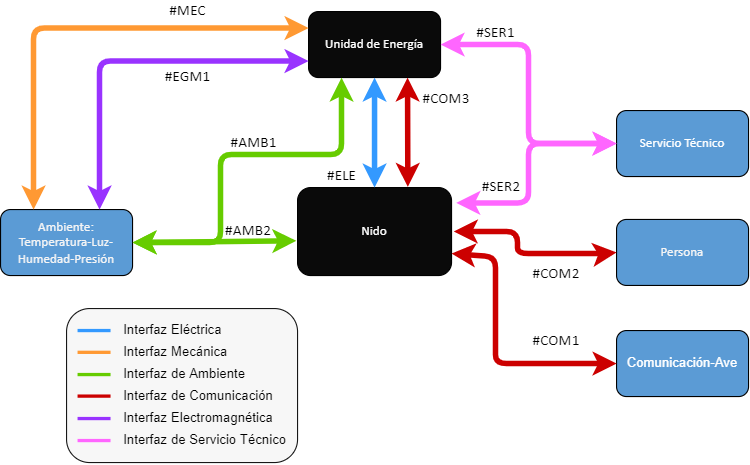
\includegraphics[width=\linewidth,page=1]{ImagenesDefinicion/func2}
	\caption{Diagrama Funcional de Interfaces.}
	\label{fig:diagrama_func_interfaces}
\end{figure}

\Subsection{Especificaciones de Diseño}
\label{sec:EspecificacionesDiseño}
\Subsubsection{Especificaciones Funcionales}
\begin{table}[H]
\centering
\begin{tabular}{|c|c|}
\hline
\multicolumn{2}{|c|}{\textbf{Leyenda para especificaciones}}    \\ \hline
\textbf{Aplicabilidad}             & \textbf{Validación}        \\ \hline
\multirow{2}{*}{P: Prototipo}      & I: Inspección Visual       \\ \cline{2-2} 
                                   & D: Documentación de Diseño \\ \hline
\multirow{2}{*}{F: Producto Final} & S: Simulación              \\ \cline{2-2} 
                                   & T: Test                    \\ \hline
\end{tabular}
\caption{Leyendas para las especificaciones.}
\end{table}

\begin{table}[H]
\centering
\begin{tabular}{|c|l|c|c|}
\hline
\textbf{ID} & \textbf{Descripción}                                                                                                                                                                                                                                                                    & \textbf{Origen}                                         & \textbf{\begin{tabular}[c]{@{}c@{}}Aplicabilidad\\ Validación\end{tabular}} \\ \hline
INT-FUN-01  & \begin{tabular}[c]{@{}l@{}}El dispositivo deberá tener un espacio de almacenamiento\\ de datos de un tamaño entre 32 a 64 GBy.\end{tabular}                                                                                                                                             & REQ-07                                                  & P F - D                                                                     \\ \hline
INT-FUN-02  & \begin{tabular}[c]{@{}l@{}}El producto debe ser capaz de obtener la temperatura\\ del entorno.\end{tabular}                                                                                                                                                                             & REQ-04                                                  & P F - I D T                                                                 \\ \hline
INT-FUN-03  & \begin{tabular}[c]{@{}l@{}}El producto debe ser capaz de obtener la humedad del\\ entorno.\end{tabular}                                                                                                                                                                                 & REQ-04                                                  & P F - I D T                                                                 \\ \hline
INT-FUN-04  & \begin{tabular}[c]{@{}l@{}}El producto debe ser capaz de obtener la intensidad\\ lumínica del interior del nido.\end{tabular}                                                                                                                                                           & REQ-04                                                  & P F - I D T                                                                 \\ \hline
INT-FUN-05  & \begin{tabular}[c]{@{}l@{}}El producto debe ser capaz de obtener video del interior\\ del nido.\end{tabular}                                                                                                                                                                            & REQ-04                                                  & P F - I D T                                                                 \\ \hline
INT-FUN-06  & \begin{tabular}[c]{@{}l@{}}El producto debe ser capaz de obtener imágenes del\\ interior del nido.\end{tabular}                                                                                                                                                                         & REQ-04                                                  & P F - I D T                                                                 \\ \hline
INT-FUN-07  & \begin{tabular}[c]{@{}l@{}}El producto debe ser capaz de detectar la presencia\\ del ave en el nido.\end{tabular}                                                                                                                                                                       & REQ-04                                                  & P F - I D T                                                                 \\ \hline
INT-FUN-08  & \begin{tabular}[c]{@{}l@{}}El producto debe transmitir de manera inalámbrica\\ los datos almacenados en el nido a un dispositivo\\ según todas las especificaciones de la tabla\\ \textit{INT-COM2}.\end{tabular}                                                                       & REQ-08                                                  & F - D                                                                       \\ \hline
INT-FUN-09  & \begin{tabular}[c]{@{}l@{}}El producto debe recibir de manera inalámbrica datos\\ almacenados en un dispositivo ajeno al proyecto según\\ todas las especificaciones de la tabla \textit{INT-COM1}.\end{tabular}                                                                        & REQ-06                                                  & F - D                                                                       \\ \hline
INT-FUN-10  & \begin{tabular}[c]{@{}l@{}}Determinar, dentro de las limitaciones tecnológicas,\\ financieras, legales y morales, además de los requisitos\\ energéticos de la mochila, si es posible la recarga\\ inalámbrica de las baterías de la mochila.\end{tabular}                              & REQ-12                                                  & P F - D                                                                     \\ \hline
INT-FUN-11  & \begin{tabular}[c]{@{}l@{}}En caso que no sea factible una recarga inalámbrica\\ de la batería de la mochila, proponer una solución\\ alternativa que permita adquirir los datos de posición del\\ ave a lo largo del estudio.\end{tabular}                                             & REQ-15                                                  & P F - D                                                                     \\ \hline
INT-FUN-12  & \begin{tabular}[c]{@{}l@{}}El sistema deber obtener las variables a medir con una\\ frecuencia de entre 5 y 60 minutos.\end{tabular}                                                                                                                                                    & REQ-04                                                  & P F -T                                                                      \\ \hline
INT-FUN-13  & \begin{tabular}[c]{@{}l@{}}El sistema debe obtener video del nido en tiempo real\\ transmitido a una computadora ubicada a una distancia\\ que por lo menos abarque entre 3.3 y 17 metros.\end{tabular}                                                                                 & REQ-04                                                  & P F -  T                                                                    \\ \hline
INT-FUN-14  & \begin{tabular}[c]{@{}l@{}}El sistema utiliza uno o más paneles solares para cargar\\ una batería de gel de ciclo profundo.\end{tabular}                                                                                                                                                & \begin{tabular}[c]{@{}c@{}}REQ-02\\ REQ-03\end{tabular} & P F - D T                                                                   \\ \hline
INT-FUN-15  & \begin{tabular}[c]{@{}l@{}}El producto debe ser capaz de mantener registro de la\\ hora y fecha correcta luego de ser previamente\\ configurada.\end{tabular}                                                                                                                           & REQ-05                                                  & P F - T                                                                     \\ \hline
INT-FUN-16  & \begin{tabular}[c]{@{}l@{}}Ante la pérdida total de la alimentación de la unidad de\\ energía y el eventual rebastecimiento de esta, el\\ producto debe ser capaz de recuperarese, mantener\\ registro de la hora y fecha correcta luego de ser\\ previamente configurada.\end{tabular} & REQ-05                                                  & P F - T                                                                     \\ \hline
\end{tabular}
\caption{Especificaciones funcionales.}
\label{tab:intFun}
\end{table}

\Subsubsection{Especificaciones de Interfaz}
\begin{table}[H]
\centering
\begin{tabular}{|c|l|c|c|}
\hline
\textbf{ID} & \textbf{Descripción}                                                                                                                                                                                       & \textbf{Origen} & \textbf{\begin{tabular}[c]{@{}c@{}}Aplicabilidad\\ Validación\end{tabular}} \\ \hline
INT-COM1-01 & \begin{tabular}[c]{@{}l@{}}La transmisión de datos debe efectuarse por medio del\\ protocolo BLE desde el la base principal de seguimiento\\ hacia la base del nido de manera unidireccional.\end{tabular} & REQ-06          & P F - T                                                                     \\ \hline
INT-COM1-02 & \begin{tabular}[c]{@{}l@{}}La transmisión de datos se efectúa una vez al día con\\ la información almacenada en la base principal de\\ seguimiento.\end{tabular}                                           & REQ-06          & F - D                                                                       \\ \hline
INT-COM1-03 & \begin{tabular}[c]{@{}l@{}}La transmisión de datos entre el nido y la base principal\\ de seguimiento debe tener un alcance de entre por lo\\ menos uno y cinco metros.\end{tabular}                       & REQ-06          & P F - T                                                                     \\ \hline
\end{tabular}
\caption{Especificaciones de interfaz COM1.}
\label{esp:COM1}
\end{table}

\begin{table}[H]
\centering
\begin{tabular}{|c|l|c|c|}
\hline
\textbf{ID} & \textbf{Descripción}                                                                                                                                                                  & \textbf{Origen} & \textbf{\begin{tabular}[c]{@{}c@{}}Aplicabilidad\\ Validación\end{tabular}} \\ \hline
INT-COM2-01 & \begin{tabular}[c]{@{}l@{}}Esta comunicación debe descargar al dispositivo de la\\ persona todos los datos seleccionados almacenados\\ en el nido.\end{tabular}                       & REQ-08          & P F - T                                                                     \\ \hline
INT-COM2-02 & \begin{tabular}[c]{@{}l@{}}La transmisión de datos debe tener un alcance que por\\ lo menos abarque entre $3.3$ y $17 \ m$.\end{tabular}                                               & REQ-08          & P F - T                                                                     \\ \hline
INT-COM2-03 & \begin{tabular}[c]{@{}l@{}}La transmisión de datos debe ser inicializada\\ por la persona de modo manual.\end{tabular}                                                                & REQ-08          & P F - D                                                                     \\ \hline
INT-COM2-04 & \begin{tabular}[c]{@{}l@{}}La transmisión de datos debe efectuarse por\\ medio del protocolo WiFi.\end{tabular}                                                                       & REQ-08          & P F - D                                                                     \\ \hline
INT-COM2-05 & \begin{tabular}[c]{@{}l@{}}Los datos descargados por el usuario son descartados\\ de los datos almacenados en el nido una vez el usuario\\ se desconecte de la red WiFi.\end{tabular} & REQ-08          & F - D T                                                                     \\ \hline
\end{tabular}
\caption{Especificaciones de interfaz COM2.}
\label{tab:esp_com_wifi}
\end{table}

\Subsubsection{Especificaciones de Dimensionales}
\begin{table}[H]
\centering
\begin{tabular}{|c|l|c|c|}
\hline
\textbf{ID} & \textbf{Descripción}                                                                                                                                                                       & \textbf{Origen} & \textbf{\begin{tabular}[c]{@{}c@{}}Aplicabilidad\\ Validación\end{tabular}} \\ \hline
IMP-DIM-01  & \begin{tabular}[c]{@{}l@{}}El dispositivo del nido no debe exceder las\\ siguientes dimensiones:\\ Largo \textless $26 \ cm$\\ Ancho \textless $8.79 \ cm$\\ Alto \textless $4.55 \ cm$\end{tabular} & REQ-01          & F - T                                                                       \\ \hline
IMP-DIM-02  & \begin{tabular}[c]{@{}l@{}}La unidad de energía no debe exceder las\\ siguientes dimensiones:\\ Largo \textless $1 \ m$\\ Ancho \textless $50 \ cm$\\ Alto \textless  $1 \ m$\end{tabular}           & REQ-01          & F - D T                                                                     \\ \hline
IMP-DIM-03  & \begin{tabular}[c]{@{}l@{}}El equipo dentro del nido no debe exceder\\ los $500 \ g$.\end{tabular}                                                                                      & REQ-01          & F - D T                                                                     \\ \hline
IMP-DIM-04  & \begin{tabular}[c]{@{}l@{}}La unidad de energía no debe exceder\\ los $20 \ kg$.\end{tabular}                                                                                             & REQ-01          & F - D T                                                                     \\ \hline
\end{tabular}
\caption{Especificaciones dimensionales y de peso.}
\label{esp:DimPeso}
\end{table}

\Subsubsection{Especificaciones de Implementación}
\begin{table}[H]
\centering
\begin{tabular}{|c|l|c|c|}
\hline
\textbf{ID} & \multicolumn{1}{c|}{\textbf{Descripción}}                                                                                                                                                                                                                             & \textbf{Origen} & \textbf{\begin{tabular}[c]{@{}c@{}}Aplicabilidad\\ Validación\end{tabular}} \\ \hline
IMP-OPE-01  & \begin{tabular}[c]{@{}l@{}}El sistema debe operar normalmente cuando la \\ temperatura  ambiente sea -20°C \textless $\text{T}_{\text{AMB}}$ \textless 30°C.\end{tabular}                                                                                           & REQ-10          & F - D                                                                       \\ \hline
IMP-OPE-02  & \begin{tabular}[c]{@{}l@{}}Debe operar normalmente cuando la humedad  sea: \\ 0\% \textless RH \textless 100\%\end{tabular}                                                                                                                                           & REQ-10          & F - D                                                                       \\ \hline
IMP-OPE-03  & \begin{tabular}[c]{@{}l@{}}El dispositivo debe operar normalmente cuando la presión \\ atmosférica sea: 84 kPa \textless $\text{P}_{\text{ATM}}$ \textless 90 kPa.\\ Esto equivale a 1500 m de altura para el mínimo de\\ presión, y un máximo de 0 m.\end{tabular} & REQ-10          & F - D                                                                       \\ \hline
IMP-DIM-04  & \begin{tabular}[c]{@{}l@{}}La unidad de energía no deberá exceder\\ los 20 kilos.\end{tabular}                                                                                                                                                                        & REQ-01          & F - D T                                                                     \\ \hline
\end{tabular}
\caption{Especificaciones de operación.}
\label{esp:OP}
\end{table}

\begin{table}[H]
\centering
\begin{tabular}{|c|l|c|c|}
\hline
\textbf{ID} & \multicolumn{1}{c|}{\textbf{Descripción}}                                                                                                                                                    & \textbf{Origen}                                         & \textbf{\begin{tabular}[c]{@{}c@{}}Aplicabilidad\\ Validación\end{tabular}} \\ \hline
IMP-AYT-01  & \begin{tabular}[c]{@{}l@{}}No se deben sufrir daños cuando, estando\\ desenergizado, la temperatura ambiente\\ sea -20°C \textless $\text{T}_{\text{AMB}}$ \textless 40°C.\end{tabular}    & \begin{tabular}[c]{@{}c@{}}REQ-10\\ REQ-13\end{tabular} & F - D                                                                       \\ \hline
IMP-AYT-02  & \begin{tabular}[c]{@{}l@{}}No se deben sufrir daños cuando, estando\\ desenergizado, la humedad\\ sea 0\% \textless RH \textless 100\%.\end{tabular}                                         & \begin{tabular}[c]{@{}c@{}}REQ-10\\ REQ-13\end{tabular} & F - D                                                                       \\ \hline
IMP-AYT-03  & \begin{tabular}[c]{@{}l@{}}No se deben sufrir daños cuando, estando\\ desenergizado, la presión atmosférica\\ sea 84 kPa \textless $\text{P}_{\text{ATM}}$ \textless 101 kPa.\end{tabular} & \begin{tabular}[c]{@{}c@{}}REQ-10\\ REQ-13\end{tabular} & F - D                                                                       \\ \hline
\end{tabular}
\caption{Especificaciones de almacenamiento y transporte.}
\label{esp:almytrans}
\end{table}

\begin{table}[H]
\centering
\begin{tabular}{|c|l|c|c|}
\hline
\textbf{ID} & \textbf{Descripción}                                                                                 & \textbf{Origen} & \textbf{\begin{tabular}[c]{@{}c@{}}Aplicabilidad\\ Validación\end{tabular}} \\ \hline
RAM-CON-01  & \begin{tabular}[c]{@{}l@{}}El producto debe tener una vida útil no\\ menor a tres años.\end{tabular} & REQ-14          & F - D                                                                       \\ \hline
\end{tabular}
\caption{Especificaciones de confiabilidad.}
\label{esp:Conf}
\end{table}

\begin{table}[H]
\centering
\begin{tabular}{|c|l|c|c|}
\hline
\textbf{ID} & \textbf{Descripción}                                                                                                                                            & \textbf{Origen} & \textbf{\begin{tabular}[c]{@{}c@{}}Aplicabilidad\\ Validación\end{tabular}} \\ \hline
RAM-SEG-01  & \begin{tabular}[c]{@{}l@{}}El dispositivo cuenta con un sistema de autenticación\\ ante el pedido de transmisión de datos definido\\ por INT-COM2.\end{tabular} & REQ-08          & P F - I D                                                                   \\ \hline
RAM-SEG-02  & \begin{tabular}[c]{@{}l@{}}El dispositivo no pose luces ni elementos reflectantes\\ para no ser percibido.\end{tabular}                                         & REQ-09          & F - I                                                                       \\ \hline
\end{tabular}
\caption{Especificaciones de seguridad.}
\label{esp:SEG}
\end{table}

\begin{table}[H]
\centering
\begin{tabular}{|c|l|c|c|}
\hline
\textbf{ID} & \textbf{Descripción}                                                                                                 & \textbf{Origen} & \textbf{\begin{tabular}[c]{@{}c@{}}Aplicabilidad\\ Validación\end{tabular}} \\ \hline
IMP-COS-01  & \begin{tabular}[c]{@{}l@{}}El costo del producto debe ser menor o igual\\ a \precio USD.\end{tabular} & REQ-11          & F - D                                                                       \\ \hline
\end{tabular}
\caption{Especificaciones de costo.}
\label{esp:COST}
\end{table}

